
%(BEGIN_QUESTION)
% Copyright 2010, Tony R. Kuphaldt, released under the Creative Commons Attribution License (v 1.0)
% This means you may do almost anything with this work of mine, so long as you give me proper credit

Suppose a 12-bit DAC (digital-to-analog converter) in a PLC analog output card has a digital range of 0 to 4095 counts (decimal) and an analog range of 0 to 20 milliamps:

$$\includegraphics[width=15.5cm]{i00737x01.eps}$$

Suppose the valve stem position is seen to be at 5\% when the analog channel register value is 604 counts (hexadecimal).  A technician measures the DC voltage appearing at the I/P converter terminals, and gets a measurement of 1.18 volts.  

\vskip 10pt

First, calculate the correct valve position corresponding to this register value.  Next, identify the likelihood of each specified fault for this circuit.  Consider each fault one at a time (i.e. no coincidental faults), determining whether or not each fault could independently account for {\it all} measurements and symptoms in this circuit.

% No blank lines allowed between lines of an \halign structure!
% I use comments (%) instead, so that TeX doesn't choke.

$$\vbox{\offinterlineskip
\halign{\strut
\vrule \quad\hfil # \ \hfil & 
\vrule \quad\hfil # \ \hfil & 
\vrule \quad\hfil # \ \hfil \vrule \cr
\noalign{\hrule}
%
% First row
{\bf Fault} & {\bf Possible} & {\bf Impossible} \cr
%
\noalign{\hrule}
%
% Another row
Open wire between ``I OUT 0'' and ``+'' terminals &  &  \cr
%
\noalign{\hrule}
%
% Another row
Open wire between ``ANL COM'' and ``$-$'' terminals &  &  \cr
%
\noalign{\hrule}
%
% Another row
I/P mis-calibration &  &  \cr
%
\noalign{\hrule}
%
% Another row
Shorted cable between PLC and I/P &  &  \cr
%
\noalign{\hrule}
%
% Another row
Defective analog output card in PLC &  &  \cr
%
\noalign{\hrule}
%
% Another row
Valve V1 shut &  &  \cr
%
\noalign{\hrule}
%
% Another row
Valve V2 shut &  &  \cr
%
\noalign{\hrule}
%
% Another row
I/P restrictor plugged (completely or partially) &  &  \cr
%
\noalign{\hrule}
%
% Another row
I/P nozzle plugged (completely or partially) &  &  \cr
%
\noalign{\hrule}
} % End of \halign 
}$$ % End of \vbox

Finally, identify the {\it next} diagnostic test or measurement you would make on this system.  Explain how the result(s) of this next test or measurement help further identify the location and/or nature of the fault.

\vfil 

\underbar{file i00737}
\eject
%(END_QUESTION)





%(BEGIN_ANSWER)

This is a graded question -- no answers or hints given!

%(END_ANSWER)





%(BEGIN_NOTES)

A count value of 604 hexadecimal is 1540 decimal.  Given a full-count range of 4095, this equates to 7.52 milliamps of signal current, which is just under 25\%.  To be exact, 7.52 mA equates to 22\%.  As the control valve is only 5\% open right now, there is definitely a problem!

\vskip 10pt

1.18 volts across an I/P resistance of 157 ohms yields a current value of 7.52 mA, which is exactly what we predicted from the given DAC count value.  This tells us we actually do have 7.52 mA going to the I/P, and that the PLC's analog output card must therefore be functioning properly.  The only possibilities for faults include something mechanically or pneumatically wrong from the I/P on to the valve.

% No blank lines allowed between lines of an \halign structure!
% I use comments (%) instead, so that TeX doesn't choke.

$$\vbox{\offinterlineskip
\halign{\strut
\vrule \quad\hfil # \ \hfil & 
\vrule \quad\hfil # \ \hfil & 
\vrule \quad\hfil # \ \hfil \vrule \cr
\noalign{\hrule}
%
% First row
{\bf Fault} & {\bf Possible} & {\bf Impossible} \cr
%
\noalign{\hrule}
%
% Another row
Open wire between ``I OUT 0'' and ``+'' terminals &  & $\surd$ \cr
%
\noalign{\hrule}
%
% Another row
Open wire between ``ANL COM'' and ``$-$'' terminals &  & $\surd$ \cr
%
\noalign{\hrule}
%
% Another row
I/P mis-calibration & $\surd$ &  \cr
%
\noalign{\hrule}
%
% Another row
Shorted cable between PLC and I/P &  & $\surd$ \cr
%
\noalign{\hrule}
%
% Another row
Defective analog output card in PLC &  & $\surd$ \cr
%
\noalign{\hrule}
%
% Another row
Valve V1 shut &  & $\surd$ \cr
%
\noalign{\hrule}
%
% Another row
Valve V2 shut & $\surd$ &  \cr
%
\noalign{\hrule}
%
% Another row
I/P restrictor plugged (completely or partially) & $\surd$ &  \cr
%
\noalign{\hrule}
%
% Another row
I/P nozzle plugged (completely or partially) &  & $\surd$ \cr
%
\noalign{\hrule}
} % End of \halign 
}$$ % End of \vbox

We know that valve V1 cannot be completely shut because if that were the case the control valve wouldn't be opening up at all.  Being 5\% open tells us there must at least be {\it some} amount of air pressure making it to the I/P and to the valve's actuating diaphragm.

\vskip 10pt

A good ``next step'' would be to manually stimulate the I/P's flapper/nozzle assembly to try to make it output full pressure.  If this works, and it makes the valve open fully, the problem is likely calibration or some other mechanical issue inside the I/P.  If a manual stimulation test does nothing, we are either dealing with a severe fault inside the I/P, a shut V2 valve, or insufficient supply pressure.

%INDEX% Electronics review: conversions to and from hexadecimal
%INDEX% Electronics review: DAC output signal calculation

%(END_NOTES)

